
\subsection{Correlation between reality and model}


\begin{figure}[H]
\small{
\begin{tabular}{p{0.32\textwidth} p{0.4\textwidth} p{0.21\textwidth}}
\textbf{Item}			& \textbf{Reality}	&  \textbf{Model}\\
\midrule
Time			& 1s		& 1 iteration\\
Maximum speed	& 120  km/h (we defined vmax as 100 km/h to get even values) & 5 (only 6 levels)\\
Length of an average car (Skoda Octavia) & 4.5 m & 1 cell\\
Distance Erstfeld - Göschenen & 19'000 m & 4222 cells (19'000 m / 4.5 m, rounded)
\end{tabular}
\caption{Units}
}
\end{figure}

\begin{figure}[H]
\small{
\begin{tabular}{p{0.22\textwidth} p{0.49\textwidth} p{0.22\textwidth}}
\textbf{Variable name}	& \textbf{Meaning}	& \textbf{Values} \\
\midrule
moveProb & Probability for a car to move forward & 0\ldots 1  \\
moveCorr & Modify moveProb for a given time (in order to improve congestion length prediction) &  -1\ldots 1\\
laneChange & Probability for a car to change its lane & 0\ldots 1\\
- & Value of laneChange as a function of distance to changeCell (for locations where cars have to change from left to right) & Constants in equation\\
redLight & Illuminate a dropcounter redlight in front of tunnel (it turns on if congestion length $>$ 2 km and redLight is set to 1) & 0, 1\\
dropCounter & Length of a period when redlight is ON & 0\ldots Inf \\
- & Maximum speed just in front of tunnel & 0\ldots 5
\end{tabular}
\caption{Variables}
}
\end{figure}


\subsection{Inflow}
The inflow is given in \#cars / 180 s. For every iteration in our model, the cars are spawned in Erstfeld (starting position) on the two lanes with a total probability $p = \#\textrm{cars} / 180$. As there are normally slightly more vehicles on the right lane, we multiply $p$ for the right lane with a factor of 1.1 and the $p$ for the left lane with a factor of 0.9.

\subsection{Average speed}
First we convert the average speed from km/h (0\ldots 120) to “Nagel-Schreckenberg-Speed” (0\ldots 5). If the speed is more than 5, we round down to 5.
Example:

Average Speed is 94 km/h. Converting into Nagel-Schreckenberg-Speed results in 4.7. Our model would in this case spawn 70\% of the cars with a speed of 5, and 30\% with a speed of 4.

\subsection{Lane Change and red-light}
As cars change lane often in reality, it should be also a part of the model. Furthermore, it is necessary to change the lane due to lane reduction in front of the tunnel. The probability to change the lane from left to the right is higher than the other way around. That yields more cars on the right lane. In front of the tunnel the probability for a lane change increases, due to lane reduction.

Red-light is activated if the congestion length exceed the length of one Kilometre. It's acting approximately 40 meters in front of the lane reduction. Every second one car can pass through the tunnel. 


\subsection{Congestion Length}
The length of a congestion is given in Kilometres. First we calculate the length of the congestion in our simulation and then multiply the length (unit: cells) by the length of a cell (4.5 m) to enable a comparison between the virtual (calculated) congestion with the real (measured) congestion.

Measuring the congestion length in our model: To obtain a stable output, we divide the highway into blocks with a length of 50 cells. If a block fulfils the two following criteria, it is declared a congestion block: high density and low average speed. We count the congestion blocks starting in Göschenen heading northbound to Erstfeld, and we only accept one uncongested block between any two blocks, otherwise we consider the congestion as terminated at the point where two or more blocks do not fulfil the congestion criteria anymore.

\subsection{Processing the datasets delivered by ASTRA}
The attached extract shows among other things that we have information about the inflow values and average speeds in 3 minutes intervals. We also have the length of the congestion at specific times (random times and course measurements). These are the three values that we used.

\begin{figure}[H]
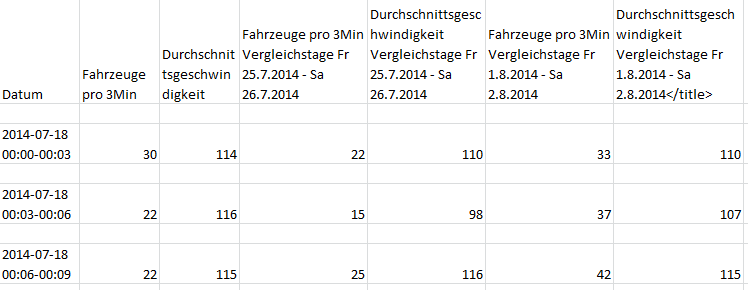
\includegraphics[width=\textwidth]{dataset.png}
\caption{Inflow values with average speeds}
\end{figure}

\begin{figure}[H]
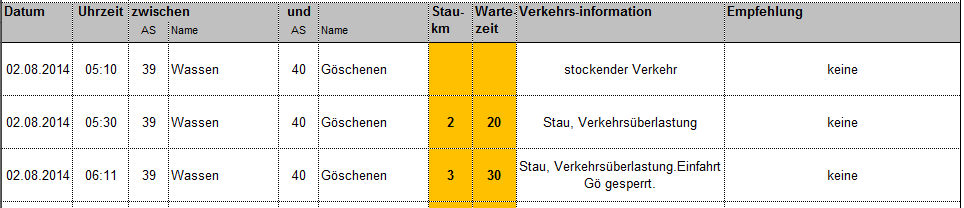
\includegraphics[width=\textwidth]{congestion.png}
\caption{Congestion data}
\end{figure}
